% This file was created by matlab2tikz.
%
%The latest updates can be retrieved from
%  http://www.mathworks.com/matlabcentral/fileexchange/22022-matlab2tikz-matlab2tikz
%where you can also make suggestions and rate matlab2tikz.
%
\definecolor{mycolor1}{rgb}{0.00000,0.44700,0.74100}%
\definecolor{mycolor2}{rgb}{0.85000,0.32500,0.09800}%
\definecolor{mycolor3}{rgb}{0.92900,0.69400,0.12500}%
%
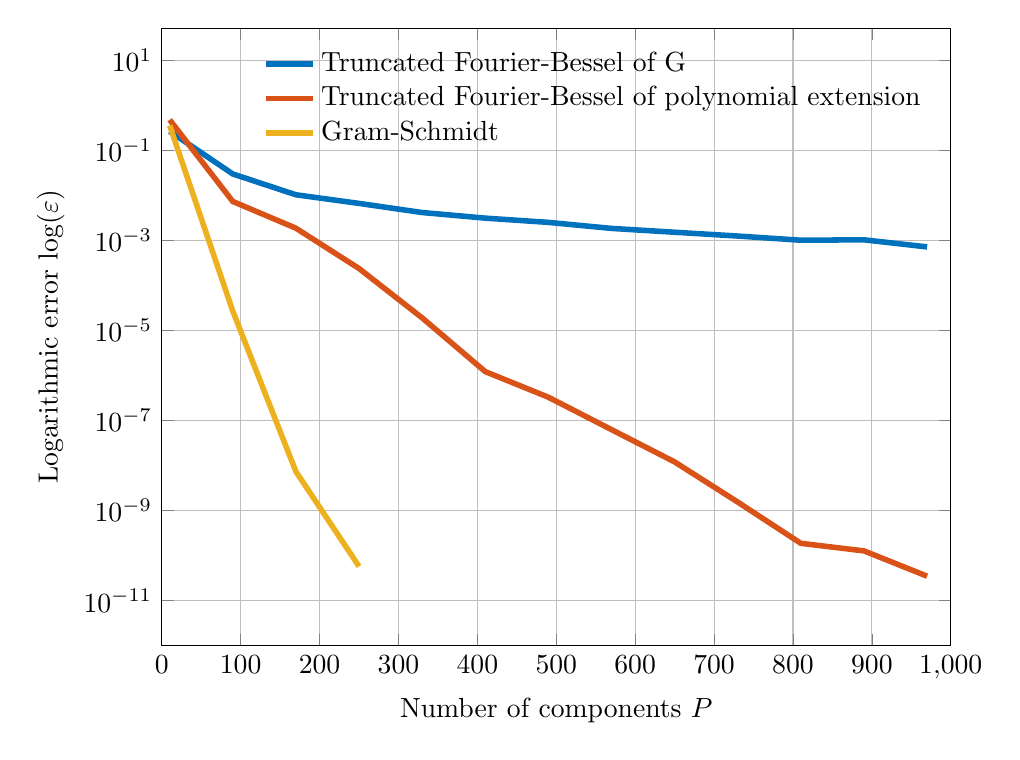
\begin{tikzpicture}

\begin{axis}[%
width=3.945in,
height=3.088in,
at={(1.334in,0.959in)},
scale only axis,
unbounded coords=jump,
xmin=0,
xmax=1000,
xlabel={Number of components $P$},
xmajorgrids,
ymode=log,
ymin=1e-12,
ymax=51,
yminorticks=true,
ylabel={Logarithmic error $\log(\varepsilon)$},
ymajorgrids,
yminorgrids,
axis background/.style={fill=white},
legend style={legend cell align=left,align=left,fill=none,draw=none}
]
\addplot [color=mycolor1,solid,line width=2.0pt]
  table[row sep=crcr]{%
10	0.263225400198431\\
90	0.0297102534119276\\
170	0.0102576565593497\\
250	0.00659898037029327\\
330	0.0041411003149312\\
410	0.00310889454079488\\
490	0.00250207181981255\\
570	0.00183865743152056\\
650	0.00151224702639796\\
730	0.00124483332891412\\
810	0.0010059566873224\\
890	0.00102602879388058\\
970	0.000714536732337567\\
};
\addlegendentry{Truncated Fourier-Bessel of G};

\addplot [color=mycolor2,solid,line width=2.0pt]
  table[row sep=crcr]{%
10	0.473497779052663\\
90	0.00727899056456138\\
170	0.00185952657621957\\
250	0.000236952574207194\\
330	1.90122394090331e-05\\
410	1.21889799009622e-06\\
490	3.29399664877883e-07\\
570	6.28558236570598e-08\\
650	1.20776539880296e-08\\
730	1.5499921346418e-09\\
810	1.88231652487048e-10\\
890	1.27994947973775e-10\\
970	3.5145220067534e-11\\
};
\addlegendentry{Truncated Fourier-Bessel of polynomial extension};

\addplot [color=mycolor3,solid,line width=2.0pt]
  table[row sep=crcr]{%
10	0.353859623754497\\
90	2.68568085779464e-05\\
170	7.38350980356017e-09\\
250	5.79021275370906e-11\\
330	nan\\
410	nan\\
490	nan\\
570	nan\\
650	nan\\
730	nan\\
810	nan\\
890	nan\\
970	nan\\
};
\addlegendentry{Gram-Schmidt};

\end{axis}
\end{tikzpicture}%